% \chapter{Theoretical Background}
\chapter{Methodology and Numerical Model Verification}


This chapter presents the design of the feed antenna and antenna lens in Ansys HFSS, together with the methodology used to verify the resulting MIMO channel model across simulation tools. Three solution routes from two platforms are considered: Sionna-RT, a ray-tracing-based channel simulator; HFSS SBR+, which approximates propagation using high-frequency ray tracing and reports the channel in terms of S-parameters; and HFSS Hybrid, which couples the finite element method (FEM) to SBR+ ray tracing and likewise reports the channel through S-parameters. Each route evaluates a common $3\times3$ MIMO configuration, with particular emphasis on angular channel variation, so that the resulting channel-quality trends can be compared consistently. Because the two HFSS routes share the SBR+ propagation engine and the Sionna-RT model uses configured antenna patterns, this comparison is treated as cross-tool numerical verification rather than as three fully independent validations.

\section{Antenna}
\subsection{Antenna Model}
In free space, the electric far field radiated by a transmit antenna can be described as a spherical wave originating from the antenna's phase center \cite{NVIDIACorporation2026}:
\begin{equation}
\mathbf{E}_T(r, \theta_T, \varphi_T) = \sqrt{\frac{P_T G_T Z_0}{2\pi}} \frac{e^{-jk_0 r} }{r}\mathbf{F}_T(\theta_T, \varphi_T)
\end{equation}

This formulation is closely related to the classical far-field expression derived from the antenna's current distribution and vector effective length \cite{ConstantineABalanis2016}, but is instead expressed in terms of input power and gain. The parameters are defined as follows: $P_T$ is the input power delivered to the transmitting antenna; $G_T$ is its maximum gain; $Z_0$ is the free-space impedance; $\mathbf{F}_T$ is the complex vector field pattern of the antenna; the factor $1/r$ accounts for spherical spreading loss; and $e^{-jk_0 r}$ represents the propagation phase delay.

Assuming conjugate impedance matching, the input power $P_T$ delivered to an antenna with impedance $Z_T$, fed by a voltage source of complex amplitude $V_T$, is given by \cite{NVIDIACorporation2026}:
\begin{equation}
P_T = \frac{|V_T|^2}{8\Re\{Z_T\}}
\end{equation}

At the receiver, the transmitted field $\mathbf{E}_T(r)$ arrives as a locally planar incoming wave $\mathbf{E}_R$, incident on the receiving antenna from the direction $(\theta_R, \varphi_R)$. The corresponding open-circuit voltage $V_R$ induced at the antenna terminals is given by \cite{NVIDIACorporation2026}:
\begin{equation}
V_R = \sqrt{\frac{\lambda^2}{4\pi} G_R \frac{4\Re\{Z_R\}}{Z_0}} \mathbf{F}_R(\theta_R, \varphi_R)^\text{H} \mathbf{E}_R,
\end{equation}
where $\lambda$ is the wavelength; $G_R$ is the gain of the receiving antenna; $Z_R$ is its impedance; $Z_0$ is the free-space impedance; $\mathbf{F}_R$ is the complex vector field pattern of the receiving antenna; and the superscript $\text{H}$ denotes the Hermitian (conjugate) transpose, which accounts for the polarization overlap between the incoming wave and the receiving antenna.

When the polarization of the incoming wave matches that of the receiving antenna, this expression reduces to the absolute voltage magnitude:
\begin{equation}
\label{eq:VR_matched}
|V_\text{R}| = \sqrt{\frac{\lambda^2}{4\pi} G_R \frac{4\Re\{Z_\text{R}\}}{Z_0}} \|\mathbf{F}_\text{R}(\theta_\text{R}, \varphi_\text{R})\| \|\mathbf{E}_\text{R}\|.
\end{equation}

Substituting the matched-polarization voltage of \eqref{eq:VR_matched} into the standard power relation, the available received power at the output of the receiving antenna can be expressed as:
\begin{align}
    P_\text{R} &= \frac{|V_\text{R}|^2}{8\Re\{Z_\text{R}\}} \\
    &= \left(\frac{\lambda}{4\pi r}\right)^2 G_\text{R} G_\text{T} P_\text{T} \left|\mathbf{F}_\text{R}(\theta_\text{R}, \varphi_\text{R})^{\mathsf{H}} \mathbf{F}_\text{T}(\theta_\text{T}, \varphi_\text{T})\right|^2.
\end{align}
% \begin{equation}
%     P_\text{R} = \left(\frac{\lambda}{4\pi r}\right)^2 G_\text{R} G_\text{T} P_\text{T} \left|\mathbf{F}_\text{R}(\theta_\text{R}, \varphi_\text{R})^{\mathsf{H}} \mathbf{F}_\text{T}(\theta_\text{T}, \varphi_\text{T})\right|^2.
% \end{equation}

\subsection{Antenna Design}
In this thesis, a microstrip patch antenna is used as the feed behind the antenna lens. Figure~\ref{fig:patch_antenna_design} summarizes its geometry, impedance matching, and radiation characteristics. The antenna model and three-dimensional gain pattern in Figure~\ref{fig:patch_antenna_design}(a) show the orientation of the patch relative to the simulation coordinates and its dominant radiation away from the antenna surface. The simulated $S_{11}$ response in Figure~\ref{fig:patch_antenna_design}(b) exhibits a deep resonance near 38.1~GHz, reaching approximately $-35$~dB. The plotted $-10$-dB impedance-matching range extends approximately from 36.9 to 39.5~GHz; thus, the intended operating frequency of 38~GHz lies well within the matched band. The 38~GHz $\phi=90^{\circ}$ gain cut in Figure~\ref{fig:patch_antenna_design}(c) further shows a broad forward main lobe and weaker back radiation. Together, these results indicate that the patch provides suitable matching and directional illumination for the subsequent transmitarray-lens characterization.

\begin{figure}[htbp]
    \centering
    \begin{subfigure}[t]{0.66\textwidth}
        \centering
        
\includegraphics[width=\linewidth]{AntennaAndPattern.PNG}
        \caption{Patch-antenna geometry and simulated three-dimensional gain pattern.}
    \end{subfigure}

    \vspace{0.6em}

    \begin{subfigure}[t]{0.52\textwidth}
        \centering
        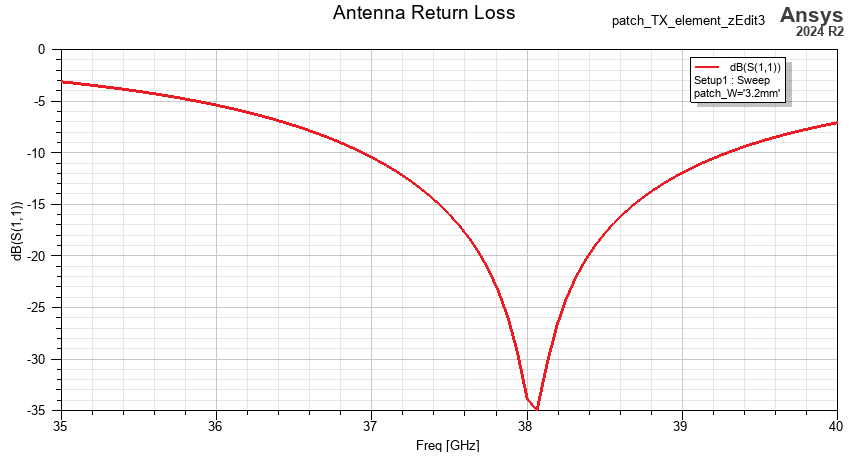
\includegraphics[width=\linewidth]{AntennaPatchReturnLoss.png}
        \caption{Simulated $S_{11}$ response from 35 to 40~GHz.}
    \end{subfigure}
    \hfill
    \begin{subfigure}[t]{0.42\textwidth}
        \centering
        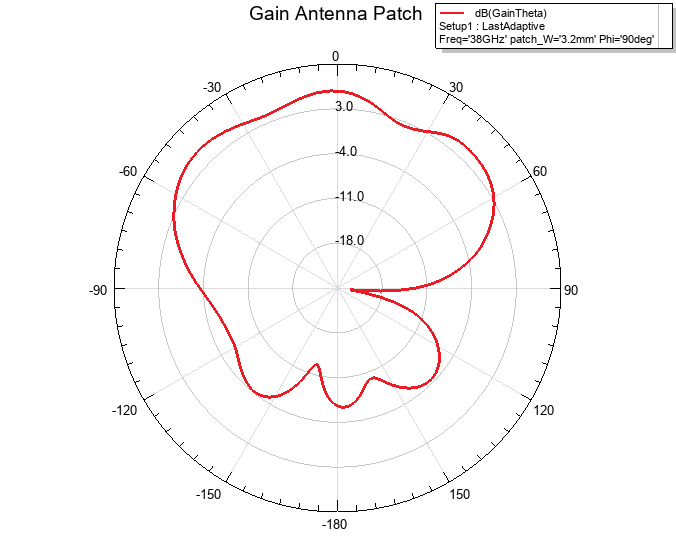
\includegraphics[width=\linewidth]{GainThetaAntennaPatch.png}
        \caption{Simulated gain cut at 38~GHz for $\phi=90^{\circ}$.}
    \end{subfigure}
    \caption{Patch feed antenna and its simulated electromagnetic performance: (a) antenna model and three-dimensional gain pattern; (b) reflection coefficient $S_{11}$; and (c) angular gain response.}
    \label{fig:patch_antenna_design}
\end{figure}

For the controlled trajectory studies in Chapter~3, the TX arrays instead use an ideal isotropic radiation pattern. This reference pattern provides uniform angular excitation and allows the comparisons to focus on the complete RX designs and order-dependent channel structure. It represents an idealized simulation source rather than a physical wire or monopole antenna.

\section{Antenna Lens Design}
% Antenna Lens Design is built on the Metasurface Transmitarray Lens Design. Also basic Theory about it.

\subsection{Metasurface Unit-Cell Design}
    \begin{figure}[htbp]
        \centering
        \begin{minipage}{0.3\textwidth}
            \centering
            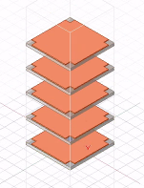
\includegraphics[width=\linewidth]{Images/Unitcell_Design.png}
            (a)
            % \label{fig:unitcell}
        \end{minipage}
        \begin{minipage}{0.48\textwidth}
            \centering
            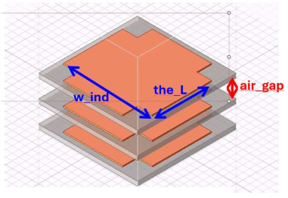
\includegraphics[width=\linewidth]{Images/Unitcell_Design_geometry.png}
            (b)
            % \label{fig:geometry}
        \end{minipage}
        \hfill        
        \caption{Unit-cell design: (a) five-layer structure with 1~mm air gaps and (b) swept geometrical dimensions.}
        \label{fig:UnitcellDesign}
    \end{figure}
    The unit-cell topology is adapted from prior work on broadband metasurface superstrates that enable polarization-independent wave focusing and gain enhancement at Ka-band frequencies~\cite{Lee2022}. As shown in Figure~\ref{fig:UnitcellDesign}, the implementation used here consists of a five-layer stacked structure separated by air gaps. Geometrical parameters, such as the patch width and layer spacing, are varied to control the transmission response.

    To evaluate the unit-cell performance, a periodic simulation setup with Floquet ports is employed, as illustrated in Figure~\ref{fig:floquet_setup}. This configuration enables the extraction of the unit-cell transmission characteristics under plane-wave excitation.

    % \centering
\begin{figure}[htbp]
     \begin{minipage}{0.24\textwidth}
         \centering
         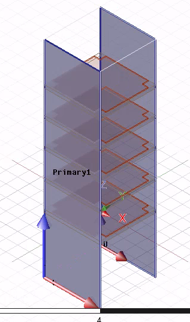
\includegraphics[width=\linewidth]{Images/FloqBoundary-1.png}
        %  \caption{Bloch Boundary 1}
        (a)
         \label{fig:floq_bound1}
     \end{minipage}
     \hfill
     \begin{minipage}{0.24\textwidth}
         \centering
         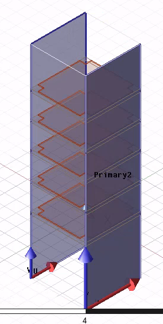
\includegraphics[width=\linewidth]{Images/FloqBoundary-2.png}
        %  \caption{Bloch Boundary 2}
        (b)
         \label{fig:floq_bound2}
     \end{minipage}
     \hfill
     \begin{minipage}{0.24\textwidth}
         \centering
         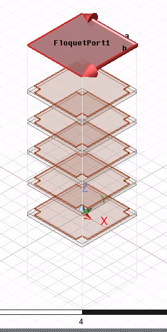
\includegraphics[width=\linewidth]{Images/FloqPort-1.png}
        %  \caption{Floquet Port 1}
         \label{fig:floq_port1}
         (c)
     \end{minipage}
     \hfill
     \begin{minipage}{0.24\textwidth}
         \centering
         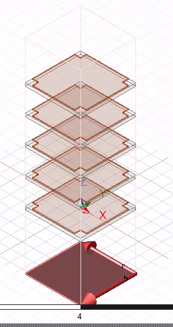
\includegraphics[width=\linewidth]{Images/FloqPort-2.png}
        %  \caption{Floquet Port 2}
         \label{fig:floq_port2}
         (d)
     \end{minipage}
     \caption{Periodic unit-cell simulation setup with Floquet boundaries and ports.}
     \label{fig:floquet_setup}
\end{figure}


    Using this simulation setup, the unit-cell geometry is swept to obtain a library of transmission responses. A candidate geometry is accepted when $S_{21,\mathrm{dB}}>-5~\mathrm{dB}$ at the 38~GHz design frequency. Applying this criterion yields 324 accepted geometries that retain usable transmitted power and provide candidate transmission phases for synthesizing the lens aperture.

    For a passive unit cell, the incident power must be accounted for by the reflected, transmitted, and dissipated components, as expressed in Equation~\ref{eq:power_conservation},
    \begin{equation}
        \left|S_{11}\right|^{2}+\left|S_{21}\right|^{2}+P_{loss}=1.
        \label{eq:power_conservation}
    \end{equation}
    From this relation, the transmitted and reflected power fractions can be expressed directly in terms of the simulated S-parameters as
    \begin{align}
        P_{T} &= \left|S_{21}\right|^{2} = 10^{\frac{S_{21,\text{dB}}}{10}}, \\
        P_{R} &= \left|S_{11}\right|^{2} = 10^{\frac{S_{11,\text{dB}}}{10}},
        \label{eq:power_definitions}
    \end{align}
    where the notation is summarized as follows:
    \begin{itemize}
        \item $S_{21}$: forward transmission coefficient;
        \item $S_{11}$: input reflection coefficient;
        \item $\left|S_{21}\right|^{2}$: transmitted-power ratio;
        \item $\left|S_{11}\right|^{2}$: reflected-power ratio;
        \item $S_{21,\text{dB}}$, $S_{11,\text{dB}}$: S-parameters expressed in decibels;
        \item $P_{T}$: transmitted-power fraction;
        \item $P_{R}$: reflected-power fraction; and
        \item $P_{\text{loss}}$: power fraction dissipated through dielectric and conductor losses.
    \end{itemize}
    At the acceptance boundary, $S_{21,\mathrm{dB}}=-5~\mathrm{dB}$ corresponds to a transmitted-power ratio of $10^{-5/10}\approx0.316$. Thus, the adopted criterion ensures that every retained geometry transmits more than approximately 31.6\% of the incident power at 38~GHz. It filters out weakly transmitting candidates, although it does not by itself separate the remaining reflected power from dielectric and conductor losses.

    Figure~\ref{fig:unitcell-accepted-library}(a) shows that the accepted geometries maintain comparatively strong transmission around the design frequency while exhibiting different frequency-dependent responses. At 38~GHz, the wrapped phases in Figure~\ref{fig:unitcell-accepted-library}(b) extend from approximately $-316^{\circ}$ to $-58^{\circ}$, corresponding to a phase span of about $258^{\circ}$. Although this span does not provide complete $360^{\circ}$ phase coverage, it offers substantially greater design flexibility than a narrowly clustered phase library. The resulting library allows the required aperture-phase profile to be approximated while preserving the $S_{21,\mathrm{dB}}>-5~\mathrm{dB}$ transmission constraint; residual phase-implementation error nevertheless remains unavoidable.

    \begin{figure}[htbp]
        \centering
        \begin{subfigure}[t]{0.96\textwidth}
            \centering
            
\includegraphics[width=\linewidth]{UnitCellProfile_Magnitude_Accepted.png}
            \caption{Transmission magnitude from 35 to 40~GHz for the 324 geometries accepted at 38~GHz.}
        \end{subfigure}

        \vspace{0.6em}

        \begin{subfigure}[t]{0.96\textwidth}
            \centering
            
\includegraphics[width=\linewidth]{UnitCellProfile_PhaseAt38GHz_Accepted.png}
            \caption{Wrapped transmission phase at 38~GHz, grouped by the swept inner-width parameter.}
        \end{subfigure}
        \caption{Transmission responses of the accepted unit-cell library: (a) magnitude response and (b) wrapped phase response at the design frequency. Only geometries satisfying $S_{21,\mathrm{dB}}>-5~\mathrm{dB}$ at 38~GHz are included.}
        \label{fig:unitcell-accepted-library}
    \end{figure}

\subsection{Lens Phase Distribution and Cell Arrangement}

The antenna lens operates by compensating for the phase variation across a spherical wavefront. When a point source is located at the focal point, its wave reaches different locations on the lens aperture after traveling different path lengths. To transform this spherical wavefront into a planar wavefront, the lens must introduce a compensating phase~\cite{Al-Joumayly2011,RezkiElArif2023}:
    \begin{equation}
        \phi(x,y) = \frac{2\pi}{\lambda_{0}}\left(\sqrt{(x-x_{f})^{2}+(y-y_{f})^{2}+f^{2}} - f\right) + \phi_{\text{init}}
        \label{eq:phase_profile}
    \end{equation}

    \noindent where
    \begin{itemize}
        \item $\phi(x,y)$ is the required phase at position $(x,y)$;
        \item $(x,y)$ are the unit-cell coordinates;
        \item $(x_{f},y_{f})$ are the transverse coordinates of the focal point relative to the aperture;
        \item $f$ is the focal distance;
        \item $\lambda_{0}$ is the free-space wavelength; and
        \item $\phi_{\text{init}}$ is the initial phase offset.
    \end{itemize}
Ideally, this phase profile aligns the transmitted waves in phase and produces a collimated beam.
The metasurface antenna lens is designed with the following parameters:

\begin{table}[h!]
	\begin{center}
		\caption{Design parameters of the metasurface antenna lens.}
		\label{table:lens_design_parameters}
		\begin{tabular}{|l|c|}
			\hline
			\textbf{Parameter} & \textbf{Value} \\
			\hline
			Unit-cell array size & $20 \times 20$ \\
			Unit-cell periodicity used in aperture calculation & $2.367\,\text{mm} \times 2.367\,\text{mm}$ \\
            Nominal aperture implied by the $20\times20$ periodic layout & $47.34\,\text{mm} \times 47.34\,\text{mm}$ \\
			Number of layers & 5 \\
			Target focal distance & 30\,mm \\
            Simulated focal distance & 14\,mm \\
			\hline
		\end{tabular}
	\end{center}
\end{table}

The nominal aperture dimensions in Table~\ref{table:lens_design_parameters} follow from $20(2.367~\mathrm{mm})=47.34~\mathrm{mm}$ along each axis. Because a coordinate export of the complete aperture is not available in the archived files, these dimensions should be confirmed against the original HFSS model.

The continuous phase profile is implemented discretely across the aperture by assigning each location to one of the available unit-cell states. Figure~\ref{fig:antenna_lens_front_view} presents the resulting front-view state map of the $20\times20$ lens. The state indices form approximately concentric regions around the aperture center: the central cells use the lowest-index state, and progressively higher-index states are assigned toward the perimeter. This radial symmetry is consistent with compensation of the spherical path-length variation from an on-axis feed and indicates that the phase profile is centered on the physical aperture. The finite number of states converts the ideal continuous phase distribution into a realizable quantized mask.

\begin{figure}[htbp]
    \centering
    
\includegraphics[width=0.62\linewidth]{AntennaLensFrontView.PNG}
    \caption{Front view of the $20\times20$ antenna lens showing the discrete unit-cell state assignment used to approximate the required radial phase distribution.}
    \label{fig:antenna_lens_front_view}
\end{figure}

Figure~\ref{fig:antenna_lens_top_view} shows the corresponding physical top view after the state map is translated into geometries from the unit-cell database. Variations in the metallic feature size and shape across the aperture implement the required transmission-phase states. The arrangement retains the radial and fourfold symmetry of the state map, while the repeated geometries within each region show that every assigned phase state is realized using a previously characterized unit-cell design. Consequently, this physical-layout representation provides a direct link between the theoretical phase profile, its discrete state assignment, and the transmitarray geometry used in the full-wave model.

\begin{figure}[htbp]
    \centering
    
\includegraphics[width=0.62\linewidth]{AntennaLensTopView_edited.PNG}
    \caption{Top view of the physical $20\times20$ transmitarray layout, in which the geometry at each aperture position implements its assigned discrete phase state.}
    \label{fig:antenna_lens_top_view}
\end{figure}

Overall, the implemented aperture preserves the intended radial phase trend. Differences from the theoretical profile can arise from the finite set of realizable unit-cell responses, incomplete phase coverage, and the associated phase discretization.

\subsection{Focal Characteristics}
% To validate the designed transmitarray metasurface lens, a plane-wave incidence simulation is performed to assess its focusing performance under a realistic excitation scenario.

% As illustrated in Figure~6, the metasurface is illuminated by a normally incident plane wave, with the propagation vector $\mathbf{k}$ oriented perpendicular to the lens aperture and the electric field $\mathbf{E}_{0}$ polarized orthogonal to $\mathbf{k}$, thereby ensuring uniform excitation across the entire unit-cell array.

% <Gambar Setup Test Simulation>

% The resulting transmitted field distribution is then examined to evaluate the focusing performance of the lens. As shown in Figure~7, the transmitted electric field is concentrated along the propagation axis and converges toward the target focal region, indicating that the incident plane wave is successfully focused by the metasurface.

% Taken together, these results confirm that the phase distribution obtained from the explored unit-cell database is correctly realized by the transmitarray structure, yielding the intended focusing behavior and validating the overall lens design methodology.

% <Gambar Hasil Simulation>

The lens was designed for a target focal distance of $f=30\,\mathrm{mm}$ using the phase profile in Equation~\ref{eq:phase_profile}. However, the full-wave field distribution in Figure~\ref{fig:focal_point_verification} reaches its narrowest region at approximately $14\,\mathrm{mm}$, considerably closer to the aperture than the design target. The continuous phase required by Equation~\ref{eq:phase_profile} is approximated using the finite set of states available from the explored unit-cell database. This phase-realization error is one plausible contributor to the focal shift; incomplete phase coverage, amplitude nonuniformity, interelement coupling, finite-aperture effects, and the feed phase-center definition may also contribute. Because these mechanisms are not isolated through an ablation study, the focal shift cannot be attributed exclusively to phase quantization. Accordingly, 30~mm is treated as the design focal distance used to generate the phase mask, whereas 14~mm is the focal distance observed in the realized full-wave model.

\begin{figure}[htbp]
    \centering
    
\includegraphics[width=0.7\linewidth]{AntennaLens20x20_VerifFocalPoint.png}
    \caption{Simulated electric-field distribution of the $20\times20$ antenna lens used to identify the axial focal point.}
    \label{fig:focal_point_verification}
\end{figure}

To further characterize the focusing behavior of the lens, its response is evaluated under oblique plane-wave incidence, with the incident angle swept from $0^\circ$ to $-60^\circ$ in steps of $15^\circ$. Figure~\ref{fig:focal_characteristics} shows the resulting field-intensity distribution behind the lens aperture for each incident angle.

\begin{figure}[htbp]
    \centering
    \begin{minipage}{0.19\textwidth}
        \centering
        
\includegraphics[width=\linewidth]{FocalCharacter_0deg.png}
        (a) $0^\circ$
    \end{minipage}
    \hfill
    \begin{minipage}{0.19\textwidth}
        \centering
        
\includegraphics[width=\linewidth]{FocalCharacter_m15degdeg.png}
        (b) $-15^\circ$
    \end{minipage}
    \hfill
    \begin{minipage}{0.19\textwidth}
        \centering
        
\includegraphics[width=\linewidth]{FocalCharacter_m30deg.png}
        (c) $-30^\circ$
    \end{minipage}
    \hfill
    \begin{minipage}{0.19\textwidth}
        \centering
        
\includegraphics[width=\linewidth]{FocalCharacter_m45deg.png}
        (d) $-45^\circ$
    \end{minipage}
    \hfill
    \begin{minipage}{0.19\textwidth}
        \centering
        
\includegraphics[width=\linewidth]{FocalCharacter_m60deg.png}
        (e) $-60^\circ$
    \end{minipage}
    \caption{Focal-plane field-intensity distribution behind the antenna lens for plane-wave incidence at (a) $0^\circ$, (b) $-15^\circ$, (c) $-30^\circ$, (d) $-45^\circ$, and (e) $-60^\circ$.}
    \label{fig:focal_characteristics}
\end{figure}

At normal incidence ($0^\circ$), the focal spot forms on the boresight axis behind the lens, consistent with the focusing behavior discussed above. As the incidence becomes more oblique, the focal region shifts progressively away from boresight while remaining at an approximately constant radial distance from the lens. The observed locus therefore resembles a focal arc rather than a single fixed point. This behavior is consistent with that of a transmitarray lens having a fixed phase profile: because the phase mask is optimized for one design incidence direction, oblique illumination relocates the focal region. Figure~\ref{fig:focal_characteristics} also shows that the focal spot becomes less distinct as the magnitude of the incidence angle increases. In particular, the responses from $-30^\circ$ to $-60^\circ$ exhibit more diffuse or multiple intensity peaks and stronger sidelobe energy than the more clearly defined focal spots at $0^\circ$ and $-15^\circ$. Thus, the simulated lens focuses waves arriving over the evaluated angular range, but its focusing quality is highest near the design incidence direction and degrades at wider oblique angles.

\subsection{Antenna Radiation Characterization}

Before presenting the simulated results, the analytical model underlying the transmitarray far-field pattern is summarized. Figure~\ref{fig:transmitarray_coord_system} defines the coordinate system. The feed is located at position vector $\vec{r}_f$ and illuminates the $(m,n)$-th transmitarray element at $\vec{r}_{mn}$ with feed-incidence angle $\theta_f(m,n)$. The far field is observed along direction $\hat{\boldsymbol{u}}$, which makes an angle $\theta_e$ with the array normal; the intended main-beam direction is denoted by $\hat{\boldsymbol{u}}_0$. Under this geometry, the complex far-field pattern of an $M\times N$ transmitarray is given by
\begin{equation}
    \begin{aligned}
        E(\theta,\varphi)
        &= \sum_{m=1}^{M}\sum_{n=1}^{N}
        \cos^{q_e}(\theta)\,
        \frac{\cos^{q_f}\!\left(\theta_f(m,n)\right)}
        {\left|\vec{r}_{mn}-\vec{r}_{f}\right|} \\[4pt]
        &\quad \times
        \exp\!\left\{-jk\left(
        \left|\vec{r}_{mn}-\vec{r}_{f}\right|
        -\vec{r}_{mn}\cdot\hat{\boldsymbol{u}}
        \right)\right\}
        \left|T_{mn}\right|e^{j\psi_{mn}},
    \end{aligned}
    \label{eq:transmitarray_pattern}
\end{equation}
where $\theta$ and $\varphi$ specify the observation direction $\hat{\boldsymbol{u}}$; $q_e$ and $q_f$ control the element and feed pattern factors, respectively; $k=2\pi/\lambda$ is the free-space wavenumber; and $|T_{mn}|e^{j\psi_{mn}}$ is the complex transmission coefficient (magnitude and phase) applied by the $(m,n)$-th element. The total radiation pattern is thus the coherent sum of every element's contribution, each weighted by its feed illumination, its own element/feed pattern factors, the free-space path loss $1/\left|\vec{r}_{mn}-\vec{r}_{f}\right|$, and the propagation phase accumulated from the feed to the element and from the element toward the observation direction. This model is the basis on which the HFSS-simulated RX lens patterns discussed below are interpreted.

\begin{figure}[htbp]
    \centering
    
\includegraphics[width=0.6\linewidth]{AntennaLensRadiationPatternAsset/TransmitArray_CoorSystem.PNG}
    \caption{Coordinate system used for the transmitarray far-field model, showing the feed, the $(m,n)$-th element, and the observation direction relative to the main-beam direction $\hat{\boldsymbol{u}}_0$.}
    \label{fig:transmitarray_coord_system}
\end{figure}

The receive (RX) antenna behind the lens is further characterized through its HFSS far-field response at $f=38~\mathrm{GHz}$. By reciprocity, the simulated transmit-mode far-field patterns can be used to characterize the receive angular response of the same passive, linear structure under consistent polarization and reference conditions. Different focal-plane antenna positions, represented by their lens-angle states, correspond to different effective aperture-phase distributions and redirect the dominant radiation region. Figure~\ref{fig:radiation_pattern_3d} presents representative three-dimensional patterns spanning the boresight and oblique configurations, whereas Figure~\ref{fig:radiation_pattern_vertical_cut} provides a quantitative X--Z-plane comparison for the boresight and negative-angle states.

The normalized three-dimensional surfaces in Figure~\ref{fig:radiation_pattern_3d} show that changing the focal-plane state displaces the dominant lobe and alters the secondary-lobe structure. The boresight and moderate-angle states retain a comparatively distinct dominant beam, whereas the widest-angle patterns become less regular, consistent with the off-axis focal spreading observed in Figure~\ref{fig:focal_characteristics}. The rectangular cuts in Figure~\ref{fig:radiation_pattern_vertical_cut} show the steering trend more clearly. Under the plotted convention $-90^\circ=+Z$, $0^\circ=+X$, and $+90^\circ=-Z$, the dominant peak moves progressively from approximately $0^\circ$ for the RX $0^\circ$ state to approximately $-55^\circ$ for the RX $-60^\circ$ state. The peak gain is about 16~dB for the boresight and moderate-angle states and decreases to approximately 12~dB for the widest RX state of $-60^\circ$. Thus, the lens supports angle-dependent beam redirection, but the increased ripple, stronger secondary lobes, and reduced peak gain at wide scan angles indicate an off-axis performance trade-off. This behavior is consistent with the finite phase coverage, phase discretization, and nonuniform aperture illumination of the realized transmitarray.

\begin{figure}[htbp]
    \centering
    
\includegraphics[width=0.95\linewidth]{AntennaPatternWithLens.png}
    \caption[Lens-assisted RX far-field patterns at 38~GHz.]{Normalized three-dimensional far-field radiation patterns at 38~GHz for representative lens-assisted RX states of $-45^\circ$, $0^\circ$, $+15^\circ$, $+30^\circ$, $+45^\circ$, and $+60^\circ$, displayed over a 40~dB dynamic range.}
    \label{fig:radiation_pattern_3d}
\end{figure}

\begin{figure}[htbp]
    \centering
    
\includegraphics[width=0.9\linewidth]{RXAntennaRadiationPattern.png}
    \caption{Rectangular vertical gain cuts in the X--Z plane at 38~GHz for RX lens-angle states of $0^\circ$, $-15^\circ$, $-30^\circ$, $-45^\circ$, and $-60^\circ$. The shifted-angle convention is $-90^\circ=+Z$, $0^\circ=+X$, and $+90^\circ=-Z$.}
    \label{fig:radiation_pattern_vertical_cut}
\end{figure}

\section{MIMO Channel Modeling}

Consider a MIMO link with $N_T$ transmit antennas and $N_R$ receive antennas. The received signals are the superposition of the transmitted signals after propagation through the channel, together with additive noise. The corresponding system model is
\begin{equation}
    \mathbf{y} = \mathbf{H}\mathbf{x} + \mathbf{n}
    \label{eq:basicMimo}
\end{equation}

where $\mathbf{x}$ and $\mathbf{y}$ are the transmit and receive vectors, respectively, $\mathbf{H}$ is the channel matrix, and $\mathbf{n}$ is the noise vector. This model applies to several MIMO representations, including the angular-domain formulation~\cite{Tse2005,Challita2022}. In the lens-assisted configuration, the receivers are placed along the focal arc behind the antenna lens so that each matrix entry characterizes the response between a transmit direction and a focal receiver. The resulting channel is then compared with that of the corresponding configuration without the lens.

\subsection{Channel State Information Formulation}
\label{subsec:csi_formulation}
At each evaluated frequency, the channel state information (CSI) of the $N_T$-transmitter, $N_R$-receiver link is represented by the complex frequency-domain matrix
\begin{equation}
    \mathbf{H}(f)=\left[H_{ij}(f)\right]
    \in \mathbb{C}^{N_R\times N_T},
    \label{eq:csi_matrix_general}
\end{equation}
where the row index $i$ identifies the receive port and the column index $j$ identifies the transmit excitation. For the $3\times3$ angular configuration used in this verification study, the common matrix convention is
\begin{equation}
    \mathbf{H}(f)=
    \begin{bmatrix}
        H_{11}(f) & H_{12}(f) & H_{13}(f) \\
        H_{21}(f) & H_{22}(f) & H_{23}(f) \\
        H_{31}(f) & H_{32}(f) & H_{33}(f)
    \end{bmatrix}.
    \label{eq:csi_matrix_3x3}
\end{equation}
The physical meaning of the indices is summarized in Table~\ref{tab:sparam_index_mapping}. The three receivers are fixed along the focal arc behind the antenna lens, whereas each transmitter illuminates the lens from the direction associated with its corresponding receiver. Because the transmitter radius is much larger than the lens focal length, the illumination at the lens is approximated as a locally plane wave. The matrix is therefore used primarily to characterize angular selectivity rather than sensitivity to the exact transmitter--lens separation.

\begin{table}[h!]
    \centering
    \caption{Angular position and role of the receive and transmit indices in $\mathbf{H}(f)$.}
    \label{tab:sparam_index_mapping}
    \begin{tabular}{|l|c|l|}
        \hline
        \textbf{Index} & \textbf{Angular position} & \textbf{Description} \\
        \hline
        $\mathrm{rx}_1$ & $0^\circ$ & Central focal receiver \\
        $\mathrm{rx}_2$ & $+45^\circ$ & Positive-angle focal receiver \\
        $\mathrm{rx}_3$ & $-45^\circ$ & Negative-angle focal receiver \\
        \hline
        $\mathrm{tx}_1$ & $0^\circ$ & Facing $\mathrm{rx}_1$, far radius \\
        $\mathrm{tx}_2$ & $+45^\circ$ & Facing $\mathrm{rx}_2$, far radius \\
        $\mathrm{tx}_3$ & $-45^\circ$ & Facing $\mathrm{rx}_3$, far radius \\
        \hline
    \end{tabular}
\end{table}

Under this convention, $H_{ii}(f)$ is a direction-matched link, whereas $H_{ij}(f)$ with $i\neq j$ is a cross-angular link. The same canonical matrix is used for all three solvers, but its entries are obtained through two solver-specific extraction routes.

For the HFSS SBR+ and Hybrid solvers, the CSI is constructed from the complex transmission S-parameters,
\begin{equation}
    H_{ij}^{\mathrm{HFSS}}(f)
    =S(\mathrm{rx}_i,\mathrm{tx}_j;f)
    =\left.\frac{b_i(f)}{a_j(f)}\right|_{a_{k\neq j}=0},
    \label{eq:csi_hfss_sparameter}
\end{equation}
where $a_j$ is the incident wave at transmit port $j$ and $b_i$ is the received wave at receive port $i$. In SBR+, rays launched by the transmitter are traced through successive reflections and transmissions. At each ray--surface intersection, the physical-optics approximation forms equivalent currents from the local fields and evaluates the scattered field over the ray footprint $S'$ as
\begin{equation}
    \bar{E}_s = \frac{1}{4\pi}\int_{S'} dS' \left[ (\hat{n}'\cdot\bar{E})\nabla'\frac{e^{-jkR}}{R} + (\hat{n}'\times\bar{E})\nabla'\frac{e^{-jkR}}{R} - j\omega\mu_0(\hat{n}'\times\bar{H})\nabla'\frac{e^{-jkR}}{R} \right],
    \label{eq:sbr_scattered_field}
\end{equation}
where $\bar{E}$ and $\bar{H}$ are the total surface fields at the intersection, $\hat{n}'$ is the surface normal, and $R$ is the distance to the observation point. The coherently summed field from all paths reaching a receiver is projected onto its far-field polarized gain vector $\bar{g}_{\mathrm{Rx}}$ to obtain
\begin{equation}
    b_i = \frac{-j\lambda}{\sqrt{4\pi\eta_0}}\,\bar{E}\cdot\bar{g}_{\mathrm{Rx}},
    \label{eq:sbr_received_signal}
\end{equation}
and hence the S-parameter in Equation~\ref{eq:csi_hfss_sparameter}. The Hybrid solver uses the same port-based definition after coupling the full-wave FEM solution around the antenna and lens to SBR+ propagation in the surrounding room.

Sionna-RT instead constructs each CSI coefficient directly from its resolved propagation paths. For the link from $\mathrm{tx}_j$ to $\mathrm{rx}_i$, the channel impulse response is
\begin{equation}
    h_{ij}(\tau)=\sum_{\ell=1}^{N_{ij}}\alpha_{ij,\ell}\,
    \delta\!\left(\tau-\tau_{ij,\ell}\right),
    \label{eq:cir}
\end{equation}
and its Fourier transform gives
\begin{equation}
    H_{ij}^{\mathrm{Sionna}}(f)=
    \sum_{\ell=1}^{N_{ij}}\alpha_{ij,\ell}
    e^{-j2\pi f\tau_{ij,\ell}},
    \label{eq:cfr}
\end{equation}
where $\alpha_{ij,\ell}$ and $\tau_{ij,\ell}$ are the complex coefficient and delay of path $\ell$, respectively~\cite{NVIDIACorporation2026,Tse2005}. Thus, the HFSS route obtains $H_{ij}(f)$ from port-to-port transmission, whereas the Sionna-RT route obtains the corresponding canonical coefficient by coherently superposing the resolved paths.

Regardless of the extraction route, the assembled CSI matrix is used in the frequency-domain input--output model
\begin{equation}
    \mathbf{y}(f)=\mathbf{H}(f)\mathbf{x}(f)+\mathbf{n}(f),
    \label{eq:mimo_frequency_domain}
\end{equation}
where $\mathbf{x}(f)\in\mathbb{C}^{N_T\times1}$ is the transmit excitation vector, $\mathbf{y}(f)\in\mathbb{C}^{N_R\times1}$ is the received-signal vector, and $\mathbf{n}(f)$ is additive noise. Each with-lens and without-lens matrix is evaluated at the common 37, 38, and 39~GHz frequency points before applying the SVD, correlation, and capacity metrics defined below.

The resulting $\mathbf{H}(f)$ should be interpreted as an effective end-to-end channel response rather than a pure free-space propagation coefficient. In HFSS it includes the transmit and receive antennas, lens response, propagation paths, mutual coupling, impedance mismatch, and port reference planes; in Sionna-RT it includes the resolved propagation paths and the configured antenna patterns. This common CSI organization enables matrix-level comparison across solvers, although differences in their field formulations and reference quantities mean that their absolute coefficients are not assumed to be numerically identical.

\subsection{Singular Value Decomposition}
At every evaluated frequency, the $3\times3$ channel matrix $\mathbf{H}$ defined in Equation~\ref{eq:csi_matrix_3x3} is decomposed using the singular value decomposition (SVD)
\begin{equation}
    \mathbf{H} = \mathbf{U}\boldsymbol{\Sigma}\mathbf{V}^{H},
    \qquad
    \boldsymbol{\Sigma} = \operatorname{diag}(\sigma_1,\sigma_2,\sigma_3),
    \qquad
    \sigma_1\geq\sigma_2\geq\sigma_3\geq0,
    \label{eq:mimo_svd}
\end{equation}
where $\mathbf{U}$ and $\mathbf{V}$ are unitary matrices whose columns form the receive- and transmit-side eigenmode bases, and $\sigma_1,\sigma_2,\sigma_3$ are the singular values of $\mathbf{H}$. Each nonzero singular value represents the gain of an orthogonal spatial eigenchannel that can, in principle, carry a separate data stream. Whenever only the relative spatial structure of the channel is of interest, $\mathbf{H}$ is additionally evaluated after Frobenius normalization,
\begin{equation}
    \widetilde{\mathbf{H}} = \frac{\mathbf{H}}{\lVert\mathbf{H}\rVert_{\mathrm{F}}},
    \label{eq:mimo_frobenius_normalization}
\end{equation}
which rescales all three singular values by the same factor. This operation removes the overall channel-amplitude difference between the with-lens and without-lens cases while leaving the relative singular-value proportions, and hence the condition number and effective rank defined below, unchanged.

\subsection{Channel Quality Metrics}
Two scalar indicators are used to summarize how balanced the three singular values are. The condition number is the ratio of the largest to the smallest singular value,
\begin{equation}
    \kappa = \frac{\sigma_1}{\sigma_3},
    \label{eq:mimo_condition_number}
\end{equation}
so that $\kappa=1$ corresponds to three perfectly balanced spatial modes, while $\kappa\gg1$ indicates that the channel is dominated by a single mode. The effective rank is obtained by first normalizing the singular values by their total power,
\begin{equation}
    p_i = \frac{\sigma_i^{2}}{\sum_{k=1}^{3}\sigma_k^{2}},
    \qquad i=1,2,3,
    \label{eq:mimo_power_fraction}
\end{equation}
and then computing the exponential of the Shannon entropy of this power distribution,
\begin{equation}
    r_{\mathrm{eff}} = \exp\!\left(-\sum_{i=1}^{3}p_i\ln p_i\right),
    \qquad 1\leq r_{\mathrm{eff}}\leq3.
    \label{eq:mimo_effective_rank}
\end{equation}
An effective rank close to $1$ indicates that the channel is dominated by a single eigenmode, whereas a value close to $3$ indicates that all three spatial modes contribute comparable power, which is favorable for transmitting three spatial streams. Because $\kappa$ and $r_{\mathrm{eff}}$ depend only on the ratios between singular values, they take identical values whether they are computed from the raw channel $\mathbf{H}$ or the Frobenius-normalized channel $\widetilde{\mathbf{H}}$ of Equation~\ref{eq:mimo_frobenius_normalization}.

\subsection{Channel Correlation Matrix}
The similarity between the channel responses associated with different antenna elements is quantified using the normalized receive- and transmit-side Gram matrices,
\begin{equation}
    \mathbf{R}_{\mathrm{RX}} = \mathbf{D}_{\mathrm{RX}}^{-1/2}\,\mathbf{H}\mathbf{H}^{H}\,\mathbf{D}_{\mathrm{RX}}^{-1/2},
    \qquad
    \mathbf{R}_{\mathrm{TX}} = \mathbf{D}_{\mathrm{TX}}^{-1/2}\,\mathbf{H}^{H}\mathbf{H}\,\mathbf{D}_{\mathrm{TX}}^{-1/2},
    \label{eq:mimo_correlation_matrix}
\end{equation}
where $\mathbf{D}_{\mathrm{RX}}$ and $\mathbf{D}_{\mathrm{TX}}$ are diagonal matrices containing the receive- and transmit-side element powers. Consequently, $\mathbf{R}_{\mathrm{RX}}$ and $\mathbf{R}_{\mathrm{TX}}$ have unit diagonal entries, and their off-diagonal entries are normalized inner products between pairs of channel responses. The channel is summarized by the mean and maximum magnitudes of these off-diagonal entries, reported separately for the receive and transmit sides. A smaller off-diagonal magnitude indicates less-aligned channel responses, which is generally favorable for spatial multiplexing, whereas a value approaching unity indicates nearly parallel responses. Because these quantities are computed from deterministic channel matrices without ensemble averaging, they are more precisely interpreted as normalized channel coherence than as statistical correlation coefficients.

\subsection{Channel Capacity}
Assuming equal power allocation across the transmit antennas, spatially white receiver noise, and perfect channel knowledge at the receiver, the per-frequency MIMO spectral efficiency at linear reference SNR $\rho$ is
\begin{equation}
    C(\rho) = \log_2\det\!\left(\mathbf{I}_{3} + \frac{\rho}{N_T}\mathbf{H}\mathbf{H}^{H}\right)
    = \sum_{i=1}^{3}\log_2\!\left(1+\frac{\rho}{N_T}\sigma_i^{2}\right)
    \quad\text{bit/s/Hz},
    \label{eq:mimo_capacity}
\end{equation}
with $N_T=3$ transmit antennas. Unless otherwise stated, the capacity results reported in this chapter are evaluated at $\rho=100$, corresponding to a reference SNR of $20~\mathrm{dB}$. For raw channels that retain propagation loss, $\rho$ is a pre-channel reference SNR rather than the received SNR after channel attenuation. Because Equation~\ref{eq:mimo_capacity} depends on the absolute singular values rather than only on their ratios, it is, unlike $\kappa$ and $r_{\mathrm{eff}}$, sensitive to the Frobenius normalization in Equation~\ref{eq:mimo_frobenius_normalization}. Capacity computed from the raw channel $\mathbf{H}$ reflects both spatial-mode balance and absolute channel strength, whereas capacity computed from $\widetilde{\mathbf{H}}$ compares the singular-value balance at a fixed unit channel energy. The latter is therefore a normalized channel-structure metric rather than an achievable link-budget throughput. No expectation over independent random channel realizations is taken here; accordingly, this quantity is not described as ergodic capacity.

\section{HFSS-Based Electromagnetic Simulation}
This section presents the electromagnetic simulations carried out in Ansys HFSS. Both HFSS solution routes report port-to-port S-parameters, which are assembled into the common CSI matrix according to Equation~\ref{eq:csi_hfss_sparameter} and subsequently evaluated using the channel metrics defined in the preceding section.

\subsection{Simulation Setup}
The electromagnetic simulation is carried out inside an indoor room environment measuring $3~\mathrm{m}\times5~\mathrm{m}\times3~\mathrm{m}$ (height $\times$ length $\times$ width), with the floor, ceiling, and all four walls assigned a concrete material to emulate an indoor propagation environment with multipath reflections. The three-element receive array, together with the antenna lens when present, is placed near one corner of the room, while the transmit excitations are positioned at fixed locations so that both line-of-sight and reflected paths from the concrete boundaries are included. Figure~\ref{fig:room_sbr} shows this room setup for the HFSS SBR+ solver, with the inset highlighting the receive array. Figure~\ref{fig:room_hybrid} shows the corresponding HFSS Hybrid setup, with the inset highlighting the antenna lens, receive array, and transmit antenna.

\begin{figure}[htbp]
    \centering
    
\includegraphics[width=0.85\linewidth]{Room_SBR_withCloseup.png}
    \caption{Indoor room simulation environment ($3~\mathrm{m}\times5~\mathrm{m}\times3~\mathrm{m}$, concrete boundaries) used in the HFSS SBR+ solver, with a close-up of the receive antenna array.}
    \label{fig:room_sbr}
\end{figure}

\begin{figure}[htbp]
    \centering
    
\includegraphics[width=0.85\linewidth]{Room_withCloseup.png}
    \caption{Indoor room simulation environment ($3~\mathrm{m}\times5~\mathrm{m}\times3~\mathrm{m}$, concrete boundaries) used in the HFSS Hybrid solver, with a close-up of the antenna lens and antenna array.}
    \label{fig:room_hybrid}
\end{figure}

The detailed layouts of the antenna arrays, lens-assisted representation, and transmitters relative to the room are shown in Figures~\ref{fig:sbr_setup_detail}--\ref{fig:hybrid_setup_top_detail}. Figure~\ref{fig:sbr_setup_detail} shows the three-dimensional close-up used in the SBR+ route, in which the three receive elements ($\mathrm{rx}_1$--$\mathrm{rx}_3$) and three transmit elements ($\mathrm{tx}_1$--$\mathrm{tx}_3$) are represented as separate radiating bodies. In this route, the with-lens response is represented through the configured lens-assisted radiation pattern rather than through an explicitly meshed multilayer lens. Figure~\ref{fig:sbr_setup_top_detail} shows the corresponding top-view schematic: the receive array is arranged on the focal arc associated with the lens, with $\mathrm{rx}_1$ on boresight ($0^{\circ}$) and $\mathrm{rx}_2$ and $\mathrm{rx}_3$ offset by $+45^{\circ}$ and $-45^{\circ}$ about the focal point, respectively. The three transmitters $\mathrm{tx}_1$--$\mathrm{tx}_3$ are placed along their corresponding angular directions and aimed toward the receive side.

\begin{figure}[htbp]
    \centering
    
\includegraphics[width=0.6\linewidth]{SetupEnvirontment_SBR_WithLens.PNG}
    \caption[HFSS SBR+ lens-assisted array configuration.]{HFSS SBR+ solver: three-dimensional close-up of the receive array ($\mathrm{rx}_1$--$\mathrm{rx}_3$) and transmit array ($\mathrm{tx}_1$--$\mathrm{tx}_3$) for the lens-assisted radiation-pattern configuration.}
    \label{fig:sbr_setup_detail}
\end{figure}

\begin{figure}[htbp]
    \centering
    
\includegraphics[width=0.7\linewidth]{SetupEnvirontment_SBR_WithLens_TopDetails.PNG}
    \caption{HFSS SBR+ solver: top-view schematic showing the focal-arc placement of $\mathrm{rx}_1$ ($0^{\circ}$), $\mathrm{rx}_2$ ($+45^{\circ}$), and $\mathrm{rx}_3$ ($-45^{\circ}$) relative to the lens reference, together with transmitter positions $\mathrm{tx}_1$--$\mathrm{tx}_3$.}
    \label{fig:sbr_setup_top_detail}
\end{figure}

The same focal-arc arrangement is retained in the HFSS Hybrid solver, but the antenna lens is modeled explicitly as a multilayer structure within the FEM region. Figure~\ref{fig:hybrid_setup_detail} shows a three-dimensional close-up of the multilayer lens, with the receive array on one side and the transmit excitation on the other. Figure~\ref{fig:hybrid_setup_top_detail} shows the corresponding top-view schematic and the $0^{\circ}/{+45^{\circ}}/{-45^{\circ}}$ focal-arc geometry of $\mathrm{rx}_1$--$\mathrm{rx}_3$.

\begin{figure}[htbp]
    \centering
    
\includegraphics[width=0.6\linewidth]{SetupEnvirontment__WithLens_Hybrid.jpeg}
    \caption{HFSS Hybrid solver: three-dimensional close-up of the multilayer antenna lens, receive array, and transmit antenna.}
    \label{fig:hybrid_setup_detail}
\end{figure}

\begin{figure}[htbp]
    \centering
    
\includegraphics[width=0.6\linewidth]{SetupEnvirontment_WithLens_Hybrid_TopDetails.png}
    \caption{HFSS Hybrid solver: top-view schematic showing the focal-arc placement of $\mathrm{rx}_1$--$\mathrm{rx}_3$ relative to the multilayer antenna lens and transmitter.}
    \label{fig:hybrid_setup_top_detail}
\end{figure}

\subsection{HFSS SBR+ Solver}
The first HFSS route uses the SBR+ (Shooting and Bouncing Ray) solver, which approximates propagation by high-frequency ray tracing and physical optics as described in Section~\ref{subsec:csi_formulation}. The canonical $3\times3$ matrix is extracted at 37, 38, and 39~GHz for both the with-lens and without-lens configurations so that their channel structures can be compared directly.

\subsubsection{HFSS SBR+ Solver Results}
Figure~\ref{fig:sbr_power} shows the normalized power distribution across the $3\times3$ channel matrix. Without the lens, the received power is distributed comparatively broadly across the transmitter--receiver pairs. For example, at 38~GHz, the diagonal terms $H(\mathrm{rx}_i,\mathrm{tx}_i)$ carry 20.3--20.4\% of the received power each, while the off-diagonal terms carry 1.2--9.1\%. With the lens-assisted patterns, the distribution becomes strongly diagonal-dominant: the $H(\mathrm{rx}_1,\mathrm{tx}_1)$ entry alone carries 53.4--69.7\% of the power over the 37--39~GHz band, while the off-diagonal entries fall below 1.5\%. These results indicate that the lens-assisted response directs a larger fraction of the received power toward the angularly matched receiver while reducing cross-angular coupling.

\begin{figure}[htbp]
    \centering
    
\includegraphics[width=0.85\linewidth]{channel_evaluation_per_method/HFSS_SBR+_Solver/power_distribution.png}
    \caption{HFSS SBR+ solver: normalized channel power distribution with and without the antenna lens.}
    \label{fig:sbr_power}
\end{figure}

This diagonal concentration is also visible in the element-wise magnitude response in Figure~\ref{fig:sbr_magnitude}. The direction-matched terms $H(\mathrm{rx}_1,\mathrm{tx}_1)$, $H(\mathrm{rx}_2,\mathrm{tx}_2)$, and $H(\mathrm{rx}_3,\mathrm{tx}_3)$ are enhanced by up to 9.1~dB at 39~GHz, whereas cross-angular terms, such as $H(\mathrm{rx}_1,\mathrm{tx}_3)$, are suppressed by as much as 15.6~dB over the same band.

\begin{figure}[htbp]
    \centering
    
\includegraphics[width=0.85\linewidth]{channel_evaluation_per_method/HFSS_SBR+_Solver/channel_3x3_magnitude_db.png}
    \caption{HFSS SBR+ solver: $3\times3$ channel magnitude response with and without the antenna lens.}
    \label{fig:sbr_magnitude}
\end{figure}

The resulting reduction in normalized channel coherence is quantified in Figure~\ref{fig:sbr_correlation}. Without the lens, the mean off-diagonal magnitude is 0.71--0.81 on both the receive and transmit sides across 37--39~GHz, indicating strongly aligned channel responses. With the lens, the mean value decreases to 0.18--0.27 on the receive side and 0.16--0.25 on the transmit side, indicating substantially less-aligned spatial responses.

\begin{figure}[htbp]
    \centering
    
\includegraphics[width=0.85\linewidth]{channel_evaluation_per_method/HFSS_SBR+_Solver/spatial_correlation.png}
    \caption{HFSS SBR+ solver: mean off-diagonal normalized channel coherence with and without the antenna lens.}
    \label{fig:sbr_correlation}
\end{figure}

Table~\ref{table:sbr_metrics} summarizes the MIMO channel-quality metrics at the design frequency of 38~GHz. Introducing the lens reduces the condition number from 6.25 to 2.22 and raises the effective rank from 1.61 to 2.36, moving it toward the ideal value of 3 for three equally weighted modes. When each channel matrix is normalized to unit Frobenius norm to remove its overall amplitude scale, the resulting normalized channel-structure capacity increases from 8.02 to 9.92~bit/s/Hz.

\begin{table}[h!]
    \begin{center}
        \caption{HFSS SBR+ solver: MIMO channel-quality metrics at 38~GHz.}
        \label{table:sbr_metrics}
        \begin{tabular}{|l|c|c|}
            \hline
            \textbf{Metric} & \textbf{Without lens} & \textbf{With lens} \\
            \hline
            Condition number & 6.25 & 2.22 \\
            Effective rank & 1.61 & 2.36 \\
            Mean normalized coherence (RX / TX) & 0.77 / 0.77 & 0.21 / 0.19 \\
            Capacity, Frobenius-normalized (bit/s/Hz) & 8.02 & 9.92 \\
            \hline
        \end{tabular}
    \end{center}
\end{table}

\subsection{HFSS Hybrid Solver}
The same $3\times3$ configuration is re-evaluated using the HFSS Hybrid solver, which combines the finite element method (FEM) with SBR+ ray tracing to capture full-wave antenna--lens interactions together with propagation through the surrounding environment. This provides a complementary cross-check of the SBR+ pattern-based results. It is not a fully independent validation because both HFSS routes use SBR+ for room-scale propagation.

In the FEM region, the electromagnetic field on the antenna and metasurface lens is governed by the vector wave equation
\begin{equation}
    \nabla\times\left(\frac{1}{\mu_r}\nabla\times\mathbf{E}\right) - k_0^2\varepsilon_r\mathbf{E} = -j\omega\mu_0\mathbf{J}_{\text{exc}},
    \qquad k_0=\omega\sqrt{\mu_0\varepsilon_0},
    \label{eq:fem_wave_eq}
\end{equation}
which HFSS solves full-wave for both $\mathbf{E}$ and $\mathbf{H}$ within this region. To solve Equation~\ref{eq:fem_wave_eq} numerically, HFSS represents the geometry with a tetrahedral mesh and expands the field in hierarchical vector basis functions $W_n$ as
\begin{equation}
    \mathbf{E} = \sum_{n=1}^{N} x_n W_n,
    \label{eq:fem_field_expansion}
\end{equation}
which, after testing Equation~\ref{eq:fem_wave_eq} against each $W_n$ and applying Green's theorem, reduces the continuous field problem to the linear matrix equation
\begin{equation}
    \mathbf{A}\mathbf{x} = \mathbf{b},
    \label{eq:fem_matrix}
\end{equation}
where $\mathbf{A}$ encodes the meshed geometry and boundary conditions and $\mathbf{b}$ contains the port excitations; solving Equation~\ref{eq:fem_matrix} for $\mathbf{x}$ yields the coefficients of Equation~\ref{eq:fem_field_expansion} and hence the field solution around the antenna and lens. From this electric field, HFSS obtains the corresponding magnetic field through the constitutive curl relation
\begin{equation}
    \mathbf{H} = \frac{j}{\omega\mu}\nabla\times\mathbf{E},
    \label{eq:fem_h_field}
\end{equation}
so that both $\mathbf{E}_{\text{FEM}}$ and $\mathbf{H}_{\text{FEM}}$ are available at the boundary of the FEM domain.

With both field components in hand, the FEM domain is enclosed by a closed \emph{Huygens surface} $S_H$ on which they are converted into equivalent surface currents
\begin{equation}
    \mathbf{J}_H = \hat{n}\times\mathbf{H}_{\text{FEM}}, \qquad \mathbf{M}_H = -\hat{n}\times\mathbf{E}_{\text{FEM}},
    \label{eq:huygens_currents}
\end{equation}
with $\hat{n}$ the outward normal of $S_H$. Rather than the physical antenna and lens geometry, these equivalent currents act as the radiating source seen by SBR+, so $S_H$ is the interface through which the near-field antenna-lens interaction resolved by FEM is coupled into the SBR+ ray tracing that propagates the field through the rest of the room.

As shown in Figure~\ref{fig:hybrid_power}, the Hybrid route reproduces the diagonal concentration observed with SBR+. Without the lens, the received power is distributed comparatively broadly, with the diagonal terms carrying 19.3--21.7\% and the off-diagonal terms carrying 3.8--16.4\% at 37~GHz. With the lens, the $H(\mathrm{rx}_1,\mathrm{tx}_1)$ term carries 51.8--59.5\% of the received power across 37--39~GHz, while every off-diagonal term falls below 1.1\%.

\begin{figure}[htbp]
    \centering
    
\includegraphics[width=0.85\linewidth]{channel_evaluation_per_method/HFSS_Hybrid_Solver/power_distribution.png}
    \caption{HFSS Hybrid solver: normalized channel power distribution with and without the antenna lens.}
    \label{fig:hybrid_power}
\end{figure}

The corresponding element-wise magnitude response is shown in Figure~\ref{fig:hybrid_magnitude}. The lens enhances the diagonal terms by up to 10.4~dB (for $H(\mathrm{rx}_1,\mathrm{tx}_1)$ at 39~GHz) while suppressing the cross term $H(\mathrm{rx}_3,\mathrm{tx}_1)$ by as much as 23.3~dB at the same frequency. The latter reduction is larger than that predicted by the SBR+ route.

\begin{figure}[htbp]
    \centering
    
\includegraphics[width=0.85\linewidth]{channel_evaluation_per_method/HFSS_Hybrid_Solver/channel_3x3_magnitude_db.png}
    \caption{HFSS Hybrid solver: $3\times3$ channel magnitude response with and without the antenna lens.}
    \label{fig:hybrid_magnitude}
\end{figure}

Figure~\ref{fig:hybrid_correlation} shows that the mean off-diagonal channel coherence decreases from 0.39--0.56 without the lens to 0.09--0.26 with the lens over the 37--39~GHz band. The without-lens baseline is lower than that predicted by SBR+, demonstrating that the absolute coherence level depends on the solver representation; the present comparison does not isolate a single cause for this difference.

\begin{figure}[htbp]
    \centering
    
\includegraphics[width=0.85\linewidth]{channel_evaluation_per_method/HFSS_Hybrid_Solver/spatial_correlation.png}
    \caption{HFSS Hybrid solver: mean off-diagonal normalized channel coherence with and without the antenna lens.}
    \label{fig:hybrid_correlation}
\end{figure}

The corresponding channel-quality metrics at 38~GHz are summarized in Table~\ref{table:hybrid_metrics}. With the lens installed, the condition number decreases from 4.42 to 1.58 and the effective rank increases from 2.06 to 2.73. The Frobenius-normalized capacity increases from 9.04 to 10.46~bit/s/Hz, reproducing the direction of the SBR+ result under the coupled FEM--SBR+ formulation.

\begin{table}[h!]
    \begin{center}
        \caption{HFSS Hybrid solver: MIMO channel-quality metrics at 38~GHz.}
        \label{table:hybrid_metrics}
        \begin{tabular}{|l|c|c|}
            \hline
            \textbf{Metric} & \textbf{Without lens} & \textbf{With lens} \\
            \hline
            Condition number & 4.42 & 1.58 \\
            Effective rank & 2.06 & 2.73 \\
            Mean normalized coherence (RX / TX) & 0.39 / 0.56 & 0.09 / 0.13 \\
            Capacity, Frobenius-normalized (bit/s/Hz) & 9.04 & 10.46 \\
            \hline
        \end{tabular}
    \end{center}
\end{table}

Overall, both HFSS routes show that the lens-assisted response redistributes power toward the diagonal of the channel matrix, lowers the normalized channel coherence, and improves the effective rank and normalized channel-structure capacity of the evaluated $3\times3$ link. These S-parameter-based results support the simulated angular-focusing behavior associated with the phase profile in Equation~\ref{eq:phase_profile}; they do not constitute experimental validation of a fabricated lens.


\section{Cross-Tool Verification}
To assess whether the lens-associated channel trend reported in the previous section also appears in another ray-tracing platform, the same $3\times3$ configuration is evaluated using Sionna-RT. Unlike the HFSS solvers, Sionna-RT constructs each matrix entry by coherently superposing its resolved propagation paths according to Equations~\ref{eq:cir} and~\ref{eq:cfr}. The resulting coefficients are arranged using the CSI convention in Equation~\ref{eq:csi_matrix_3x3}, enabling a matrix-level comparison after harmonization. Qualitative agreement between Sionna-RT and the two HFSS routes supports a cross-tool numerical trend, but it does not constitute independent experimental validation of a physical prototype.

\subsection{Simulation Setup}
The Sionna-RT simulation reproduces the HFSS SBR+ indoor scenario: an isolated $3~\mathrm{m}\times5~\mathrm{m}\times3~\mathrm{m}$ room with $0.2~\mathrm{m}$-thick concrete walls and a nominal operating frequency of 38~GHz evaluated from 37 to 39~GHz. In the implemented workflow, the RX radiation pattern cannot be varied within a single run. The $3\times3$ channel matrix is therefore assembled from three separate ray-tracing simulations, one for each RX antenna pattern, and the results are combined into an equivalent $3\times3$ channel matrix. This construction assumes identical coordinate origins, phase centers, polarization bases, frequency grids, and complex-phase conventions across the three runs. The with-lens and without-lens antenna representations are evaluated under the same scene geometry; consequently, the comparison is between two complete antenna configurations rather than an explicit environmental scattering model of the lens.

\subsection{Simulation Results}
Figure~\ref{fig:sionna_power} shows the resulting normalized power distribution. Without the lens, the received power is more concentrated toward $\mathrm{rx}_1$ than in the HFSS results, with the diagonal terms carrying 18.0--21.6\% and several off-diagonal terms carrying 5.7--12.4\%. With the lens, the $H(\mathrm{rx}_1,\mathrm{tx}_1)$ entry carries 58.2--58.7\% of the power across 37--39~GHz, while every off-diagonal term falls below 0.4\%. Sionna-RT therefore predicts a sharper diagonal concentration than either HFSS route.

\begin{figure}[htbp]
    \centering
    
\includegraphics[width=0.85\linewidth]{channel_evaluation_per_method/SIonna-RT/power_distribution.png}
    \caption{Sionna-RT: normalized channel power distribution with and without the antenna lens.}
    \label{fig:sionna_power}
\end{figure}

The corresponding element-wise magnitude response is shown in Figure~\ref{fig:sionna_magnitude}. The lens-assisted representation enhances the three direction-matched diagonal terms by 5.2--10.7~dB, while the cross-angular terms are attenuated by 2.1--11.9~dB. This reproduces the angular-selective trend observed with the HFSS routes, although the suppression is less uniform across the individual cross terms.

\begin{figure}[htbp]
    \centering
    
\includegraphics[width=0.85\linewidth]{channel_evaluation_per_method/SIonna-RT/channel_3x3_magnitude_db.png}
    \caption{Sionna-RT: $3\times3$ channel magnitude response with and without the antenna lens.}
    \label{fig:sionna_magnitude}
\end{figure}

Figure~\ref{fig:sionna_correlation} shows the resulting normalized channel coherence. At 38~GHz, the mean off-diagonal value decreases from 0.297 (RX) / 0.335 (TX) without the lens to 0.177 (RX) / 0.181 (TX) with the lens, a reduction of approximately 40--46\%. The direction of this change agrees with the HFSS results, although Sionna-RT begins from a substantially lower without-lens baseline.

\begin{figure}[htbp]
    \centering
    
\includegraphics[width=0.85\linewidth]{channel_evaluation_per_method/SIonna-RT/spatial_correlation.png}
    \caption{Sionna-RT: mean off-diagonal normalized channel coherence with and without the antenna lens.}
    \label{fig:sionna_correlation}
\end{figure}

Table~\ref{table:sionna_metrics} summarizes the channel-quality metrics at 38~GHz. Unlike the HFSS results, the without-lens condition number (2.06) is already close to the with-lens value (1.92), and the without-lens effective rank (2.60) is marginally higher than the with-lens value (2.56). The Frobenius-normalized capacity is therefore almost unchanged (10.23 vs.\ 10.20~bit/s/Hz), because the Sionna-RT representation predicts a comparatively well-conditioned channel even without the lens. The main improvement predicted by Sionna-RT instead appears in the raw capacity, which rises from 0.317 to 1.033~bit/s/Hz. This increase reflects stronger absolute singular values under the adopted channel and reference-SNR scaling, rather than an improvement in the relative spatial-mode balance.

\begin{table}[h!]
    \begin{center}
        \caption{Sionna-RT: MIMO channel-quality metrics at 38~GHz.}
        \label{table:sionna_metrics}
        \begin{tabular}{|l|c|c|}
            \hline
            \textbf{Metric} & \textbf{Without lens} & \textbf{With lens} \\
            \hline
            Condition number & 2.06 & 1.92 \\
            Effective rank & 2.60 & 2.56 \\
            Mean normalized coherence (RX / TX) & 0.30 / 0.34 & 0.18 / 0.18 \\
            Capacity, raw, 20~dB reference SNR (bit/s/Hz) & 0.32 & 1.03 \\
            Capacity, Frobenius-normalized (bit/s/Hz) & 10.23 & 10.20 \\
            \hline
        \end{tabular}
    \end{center}
\end{table}

\subsection{Comparison Basis and Channel Harmonization}
To compare the three solution routes, the native antenna and port labels of each method are mapped to a common $3\times3$ channel convention using canonical $\mathrm{rx}_1$--$\mathrm{rx}_3$ and $\mathrm{tx}_1$--$\mathrm{tx}_3$ indices at the 37, 38, and 39~GHz anchor frequencies. The processed results are stored in \path{Images/channel_comparison_results}. This mapping is necessary because the Hybrid route uses swept incident-angle excitations, whereas Sionna-RT and SBR+ use explicit transmitter indices. Two channel forms are used in the comparison: raw complex matrices, which retain each solver's absolute channel scale, and Frobenius-normalized matrices $\widetilde{\mathbf{H}}=\mathbf{H}/\lVert\mathbf{H}\rVert_{\mathrm{F}}$, which remove that scale and isolate the relative spatial-mode structure. Raw magnitudes and capacities may be compared descriptively, but their absolute inter-solver differences also contain differences in antenna representation, reference plane, and channel normalization. Results from the raw and normalized matrices are therefore interpreted separately.

\subsection{Absolute Channel-Magnitude Comparison}
Figure~\ref{fig:comparison_channel_with_magnitude} compares the nine canonical TX--RX channel coefficients predicted by the three solvers. All three reproduce the same broad channel organization (diagonal-dominant with the lens, more evenly spread without it), but they do not predict identical absolute magnitudes, which is expected given their different field formulations, propagation approximations, antenna representations, and channel-extraction procedures.

\begin{figure}[htbp]
    \centering
    
\includegraphics[width=\linewidth]{channel_comparison_results/channel_3x3_with_magnitude_db.png}
    \caption{Inter-solver comparison of the $3\times3$ channel magnitudes at 37, 38, and 39~GHz with the antenna lens.}
    \label{fig:comparison_channel_with_magnitude}
\end{figure}

The pairwise discrepancy summary in Figure~\ref{fig:comparison_pairwise_discrepancy} quantifies this agreement. With the lens, SBR+ and Sionna-RT show the closest agreement, with a mean absolute magnitude difference of 3.66~dB and a centered frequency-shape difference of 1.46~dB, while Hybrid differs from Sionna-RT and SBR+ by 4.71~dB and 6.11~dB, respectively. Without the lens, Hybrid and Sionna-RT agree most closely, with mean magnitude and shape differences of 2.20~dB and 0.49~dB.

\begin{figure}[htbp]
    \centering
    
\includegraphics[width=0.9\linewidth]{channel_comparison_results/inter_solver_pairwise_discrepancy.png}
    \caption[Pairwise discrepancies among the three solver results.]{Mean pairwise absolute-magnitude and centered frequency-shape discrepancies among the Hybrid, SBR+, and Sionna-RT results; a smaller value indicates closer inter-solver agreement.}
    \label{fig:comparison_pairwise_discrepancy}
\end{figure}

\subsection{Lens-Effect Comparison}
Figure~\ref{fig:comparison_lens_gain} shows the lens-associated magnitude change for every canonical link, defined as
\[
    \Delta H_{ij,\mathrm{lens}}
    =H_{ij,\mathrm{with,dB}}-H_{ij,\mathrm{without,dB}}.
\]
All three solvers predict positive changes for the direction-matched diagonal links and predominantly negative changes for the off-diagonal links. Averaged over the three anchor frequencies, the diagonal changes are 8.33~dB for Hybrid, 5.33~dB for SBR+, and 7.12~dB for Sionna-RT, while the mean off-diagonal changes are $-7.58$, $-7.86$, and $-7.48$~dB, respectively.

\begin{figure}[htbp]
    \centering
    
\includegraphics[width=\linewidth]{channel_comparison_results/channel_3x3_lens_gain.png}
    \caption{Lens-associated channel-magnitude change for every canonical TX--RX pair and solver.}
    \label{fig:comparison_lens_gain}
\end{figure}

As summarized in Figure~\ref{fig:comparison_lens_direction_agreement}, the three solvers agree on the direction of the lens-associated change (increase or decrease) at 25 of the 27 link--frequency combinations (92.6\%). The only exceptions are $H(\mathrm{rx}_3,\mathrm{tx}_2)$ at 37 and 39~GHz, where two solvers predict a decrease and one predicts an increase. This descriptive sign agreement shows a consistent trend across the evaluated points, although the 27 combinations are not independent statistical trials and the percentage is not a significance test.

\begin{figure}[htbp]
    \centering
    
\includegraphics[width=0.55\linewidth]{channel_comparison_results/lens_effect_direction_agreement.png}
    \caption{Fraction of the 37, 38, and 39~GHz anchor points for which all three solvers agree on the direction of the lens-associated change.}
    \label{fig:comparison_lens_direction_agreement}
\end{figure}

\subsection{Inter-Solver MIMO Quality and Capacity}
Figure~\ref{fig:comparison_mimo_raw} and Table~\ref{table:comparison_mimo_38ghz} compare the condition number, effective rank, and raw capacity at a 20~dB reference SNR while retaining each solver's absolute channel scale.

\begin{figure}[htbp]
    \centering
    
\includegraphics[width=\linewidth]{channel_comparison_results/mimo_evaluation_raw.png}
    \caption[Raw-channel MIMO metrics across the three solvers.]{Raw-channel inter-solver MIMO evaluation at 37, 38, and 39~GHz, with the antenna lens (top row) and without it (bottom row).}
    \label{fig:comparison_mimo_raw}
\end{figure}

\begin{table}[h!]
    \begin{center}
        \caption{Raw-channel MIMO metrics at 38~GHz across the three solvers.}
        \label{table:comparison_mimo_38ghz}
        \footnotesize
        \begin{tabular}{|l|l|c|c|c|}
            \hline
            \textbf{Solver} & \textbf{Lens} & \textbf{Condition number} & \textbf{Effective rank} & \textbf{Capacity (bit/s/Hz)} \\
            \hline
            HFSS Hybrid & With    & 1.58 & 2.73 & 1.11 \\
            HFSS Hybrid & Without & 4.42 & 2.06 & 0.38 \\
            HFSS SBR+   & With    & 2.22 & 2.36 & 1.44 \\
            HFSS SBR+   & Without & 6.25 & 1.61 & 0.60 \\
            Sionna-RT   & With    & 1.92 & 2.56 & 1.03 \\
            Sionna-RT   & Without & 2.06 & 2.60 & 0.32 \\
            \hline
        \end{tabular}
    \end{center}
\end{table}

At 38~GHz, all three solvers predict a raw-capacity increase for the lens-assisted configuration: Hybrid increases from 0.38 to 1.11~bit/s/Hz, SBR+ from 0.60 to 1.44~bit/s/Hz, and Sionna-RT from 0.32 to 1.03~bit/s/Hz. Hybrid predicts the most balanced with-lens channel at this frequency ($\kappa=1.58$) and the highest effective rank (2.73), whereas SBR+ predicts the largest raw capacity (1.44~bit/s/Hz). Sionna-RT predicts the smallest change in condition number but still produces a substantial raw-capacity increase because the absolute singular values increase. Figure~\ref{fig:comparison_normalized_singular_values} separates spatial-mode balance from absolute channel scale. With the lens, all three solvers retain three visible spatial modes; without the lens, Hybrid and especially SBR+ show a comparatively weak third normalized singular value, whereas Sionna-RT already predicts a more balanced mode distribution. The raw-capacity ranking must therefore be interpreted together with the normalized spatial structure and the solver-specific channel scale.

\begin{figure}[htbp]
    \centering
    
\includegraphics[width=\linewidth]{channel_comparison_results/mimo_normalized_singular_values.png}
    \caption{Frobenius-normalized singular values for the three solvers at the common anchor frequencies.}
    \label{fig:comparison_normalized_singular_values}
\end{figure}

\subsection{Normalized Channel-Coherence Comparison}
Figure~\ref{fig:comparison_spatial_correlation} provides the most consistent matrix-level evidence of the lens-associated trend across solvers. At 38~GHz, the mean RX/TX off-diagonal coherence values with the lens are 0.085/0.126 for Hybrid, 0.213/0.188 for SBR+, and 0.177/0.181 for Sionna-RT; without the lens, the corresponding values are 0.393/0.561, 0.767/0.767, and 0.297/0.335. Every solver therefore predicts lower RX- and TX-side channel coherence for the lens-assisted configuration, although the absolute without-lens level differs substantially between solvers.

\begin{figure}[htbp]
    \centering
    
\includegraphics[width=\linewidth]{channel_comparison_results/mimo_spatial_correlation_evaluation.png}
    \caption{Mean off-diagonal RX- and TX-side normalized channel coherence for the three solvers at 37, 38, and 39~GHz, with and without the lens.}
    \label{fig:comparison_spatial_correlation}
\end{figure}

\subsection{Overall Comparison and Interpretation}
The three simulation routes---HFSS Hybrid (FEM coupled to SBR+), HFSS SBR+ (pattern-based ray tracing with S-parameters), and Sionna-RT (ray tracing with configured antenna patterns)---support the same principal qualitative result: the lens-assisted configuration strengthens the direction-matched channel entries, suppresses most cross-angular entries, increases raw capacity at the 20~dB reference SNR, and reduces normalized channel coherence. The sign of the lens-associated magnitude change agrees across all three solvers for 25 of the 27 evaluated link--frequency points, and all three predict higher raw capacity and lower coherence at the 38~GHz design frequency. These findings constitute cross-tool numerical agreement, not three independent validations.

The solvers should nevertheless not be treated as numerically interchangeable. Absolute with-lens magnitude differences remain several decibels, and the predicted condition number, effective rank, and without-lens baseline coherence differ noticeably among the methods. In particular, Sionna-RT predicts a substantially better-conditioned without-lens channel than either HFSS route. SBR+ and Sionna-RT agree most closely on the with-lens magnitude, whereas Hybrid and Sionna-RT agree most closely without the lens; Hybrid predicts the best with-lens spatial balance at 38~GHz, and SBR+ predicts the highest raw capacity. The cross-solver evidence is therefore strongest for direction-matched enhancement, cross-angular suppression, raw-capacity improvement, and reduced normalized coherence. It is weaker for a universal improvement in effective rank or Frobenius-normalized capacity, because Sionna-RT predicts a slight decrease in both of these metrics. Exact link magnitude, phase, and baseline channel conditioning remain solver-specific.

\iffalse
% TODO: outline for remaining subsections
\begin{itemize}
    \item Geometry design (explain in figure)
    \item Substrate and conductor properties (explain in figure)
    \item Periodic boundary conditions (explain in figure)
    \item Floquet-port excitation (explain in figure)
    \item Geometrical parameter sweep [connector into Transmission Phase]
    \item Transmission Phase Characterization (explain 2 figures: magnitude graph, phase graph)
    \begin{itemize}
        \item Transmission magnitude $S_{11}$ and $S_{21}$ response
        \item Wrapped and unwrapped transmission phase
        \item Available phase range
        \item Unit-cell selection criteria
    \end{itemize}
    \item Lens phase distribution / cell arrangement
    \item Formulation for generating the unit cell
    \item Focal characteristics
    \begin{itemize}
        \item Show figure of the antenna lens focusing in the near field
        \item Show results for other incidence angles for verification (need at least 2,1)
    \end{itemize}
\end{itemize}
\fi
